\chapter{Hardware}
In wat volgt, worden alle componenten uitvoerig besproken en wordt een verantwoording gegeven van de ontwerpskeuzes.

\section{Drone} \label{sec:drone}
De eerste beslissing omtrent hardware was het uitzoeken van de drone. Hier werd geopteerd voor de Parrot AR.Drone 2.0 Elite Edition met jungle camo. De belangrijkste argumenten voor deze keuze zijn de kostprijs en de grootte.\\

Vaak kosten drones die een lading van zo'n \SI{100}{\g} kunnen dragen minstens \SI{250}{\euro{}}. Dit type is echter al even niet meer in productie, waardoor de prijs enorm gezakt is. Een goedkopere drone, die niet onder de minidrones geplaatst wordt, kon niet gevonden worden.\\

Ook voor het software gedeelte is deze drone een goede keuze. Parrot stelt een SDK openbaar ter beschikking en er bestaan reeds libraries, waarvan er in dit project ook gebruik gemaakt wordt.\\
De camera op de drone zou kunnen dienen om barcodes in te scannen, maar dat onderdeel werd niet onder de doelstellingen van dit project gedefini\"eerd.\\
Tot slot bezit de drone ook nog een ultrasone sensor om de hoogte t.o.v. de vloer te meten en een camera om stabiel te blijven zweven op dezelfde positie.

\section{Indoor lokalisatie}  \label{sec:uwb}
In theorie is het mogelijk om, als een drone op een gekende locatie (met een gekende ori\"entatie) vertrekt, deze zonder enige input informatie of correcties een reeks vluchtbewegingen door te geven zodat een voorgeprogrammeerde route gevolgd wordt. In de praktijk wordt dit echter bemoeilijkt door ongekende externe factoren, denk bijvoorbeeld maar aan een ongekend obstakel dat plots het pad van de drone kruist, of een ventilatieschacht die de drone uit positie blaast. Ook het opstijgen gebeurt niet vlekkeloos, waardoor hij met een foutieve ori\"entatie aan zijn tocht zou beginnen. Daarom is het nodig dat het toestel z'n specifieke locatie in de ruimte op elk moment gekend is. \\

Als de drone tussen 2 rekken met een doorgang van \SI{1}{\m} moet kunnen vliegen, dan moet de nauwkeurigheid van lokalisatie in de grootte orde van \SI{0.10}{\m} liggen. Veelgebruikte lokalisatie-technologie\"en zoals gps, wifi en bluetooth zijn te onnauwkeurig voor deze toepassing. Ultra Wide Band komt deze noden tegemoet. Dit is een vrij recente techniek met een nauwkeurigheid in de grootteorde van \SI{0.10}{\m}, wat volstaat om de drone indoor te kunnen lokaliseren.\\

Voor de locatiebepaling werd beroep gedaan op de Pozyx-hardware\footnote{\url{https://www.pozyx.io}}, ontwikkeld door een spin-off van de Ugent, meer bepaald op de anker nodes (die op gekende locaties in de ruimte worden opgehangen) en op een mobiele tag (die als onderdeel van de controller op de drone wordt bevestigd). 
Over de mobiele tag is meer te vinden in sectie \ref{sec:pozyx_tag}.

\section{On-board Controller} \label{sec:onboard_controller}

De locatiebepaling gebeurt via een controller die we op de drone monteren, deze bestaat uit een Pozyx tag, een Raspberry Pi Zero W en een batterij.

\subsection{Pozyx tag}  \label{sec:pozyx_tag}
De mobiele tag kan om de beurt de verschillende ankers aanspreken, en opvragen hoe ver hij van hen verwijderd is. Wanneer er enkele van deze afstanden gekend zijn, kan hij zijn locatie bepalen ten opzichte van de ankers.\\

Er werden twee verschillende opties vergelijken (zie tabel \ref{tab:decavspozyx}) als mogelijke UWB component: DecaWave DWM1001 en Pozyx. De DecaWave is een goedkope, lichte en compacte module. Echter zou het implementeren van de lokalisatie geen makkelijk programmeertaak zijn, mede doordat de communicatie met de chip niet evident is. Ook waren deze module niet direct beschikbaar. Hierdoor is er gekozen voor de duurdere, zwaardere en grotere pozyx tag. Deze waren direct beschikbaar, en ook de begeleiders hadden hier reeds ervaring mee. Voor de gebruikte drone is het minieme gewichtsverschil niet echt een probleem. Men moet echter wel in het achterhoofd houden dat meer massa de stabiliteit en vliegminuten in negatieve zin be\"invloedt.\\

\begin{table}[p]
\centering
\begin{tabular}{ | l | c | c | } \hline
& DecaWave DWM1001 & Pozyx \\
\hline 
\hline
Prijs (\euro{}) & 20 & 135 \\ 
\hline
Massa (g) & 4 & 12 \\ 
\hline
Afmetingen ($mm \times mm$) & $19.1 \times 26.2$ & $60 \times 53$ \\ 
\hline
\end{tabular}
\caption[Vergelijking DecaWave DWM1001 Module en Pozyx tag]{Vergelijking DecaWave DWM1001 Module en Pozyx tag}
\label{tab:decavspozyx}
\end{table}

\subsection{Raspberry Pi Zero W} \label{sec:raspberry_pi}

Het aansturen van de Pozyx tag gebeurt met een Raspberry Pi Zero W. 

\subsection{LiPo Batterij en Power Supply} \label{sec:lipo}
De Lithium-ion Polymeer Batterij (LiPo) moet de controller gedurende ongeveer een kwartier van stroom kunnen voorzien, aangezien de drone ook ongeveer \SI{15}{\min} lang in de lucht kan blijven.\\
De controller heeft gedurende een kwartier ongeveer \SI{350}{\mA} nodig. Om pieken op te kunnen vangen werd gekozen voor een batterij van \SI{500}{\mA\hour}. Deze kan gedurende een kwartier zo'n \SI{2000}{\mA} leveren aan de controller.\\

Omdat de Rasberry Pi Zero W op \SI{5}{\V} opereert i.p.v. op de \SI{3.7}{\V} van de LiPo batterij, wordt er nog een LiPo SHIM tussen geplaatst. Deze zal niet enkel het voltage omvormen, maar bezit ook een indicator dat inschakelt wanneer de batterij bijna leeg is.

\section{Off-board Controller} \label{sec:offboard_controller}
Om de drone effectief aan te sturen maken we gebruik van een Raspberry Pi 3 B. Deze heeft de mogelijkheid om met 2 netwerken tegelijk te verbinden. De Ethernet interface wordt gebruikt om verbinding te maken met het internet (en de MQTT server), terwijl de wifi interface gebruikt wordt om met het netwerk van de drone te verbinden.

\section{Setup} \label{sec:setup_hardware}
Op figuur \ref{fig:setup_hardware} vindt u de hardware setup.
\begin{figure}[p]
	\centering
	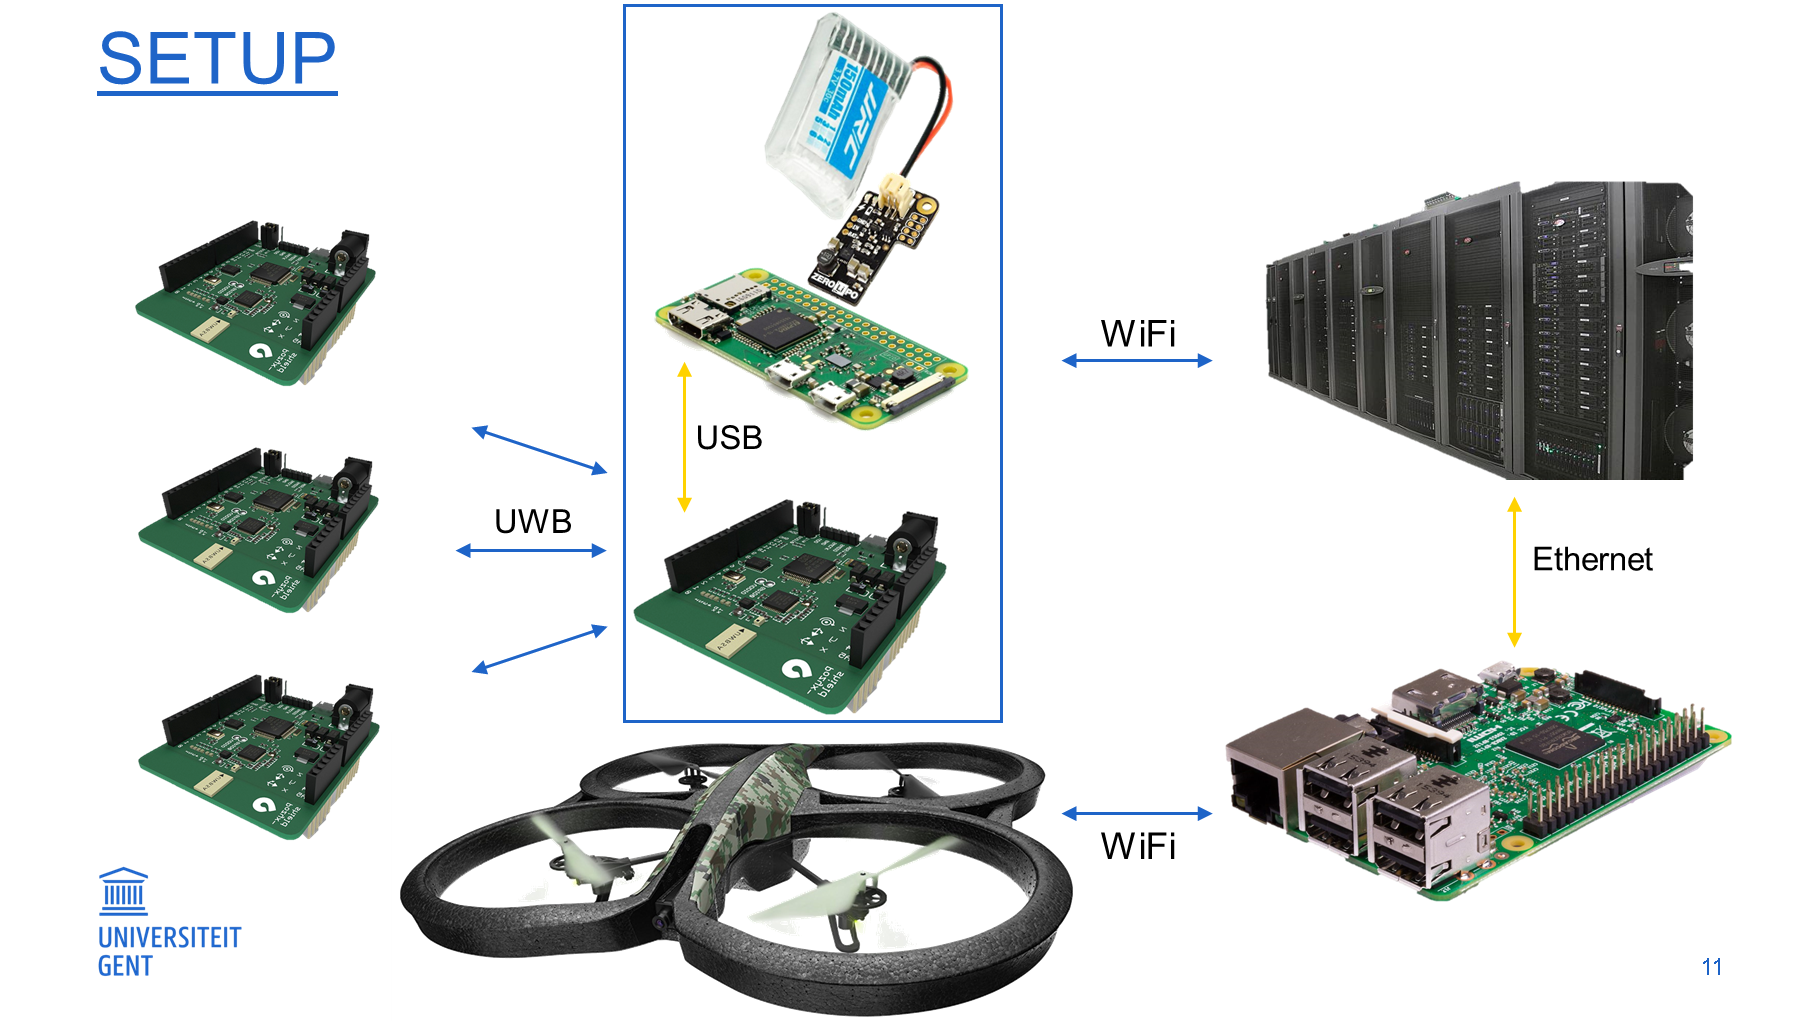
\includegraphics[width=\textwidth]{Setup_Hardware}
	\caption[Hardware setup]{Hardware setup.}
	\label{fig:setup_hardware}
\end{figure}